\normaltrue \difficilefalse \tdifficilefalse
\correctionfalse

%\UPSTIidClasse{11} % 11 sup, 12 spé
%\newcommand{\UPSTIidClasse}{12}

\exer{Poussoir $\star$ \label{C2:06:16}}
\setcounter{question}{0}\UPSTIcompetence[2]{C2-06}
\index{Compétence C2-06}
\ifcorrection
\else
\marginnote{\textbf{Pas de corrigé pour cet exercice.}}
\fi

\ifprof
\else
Soit le mécanisme suivant. On a $\vect{AC}=L\vect{i_0}+H\vect{j_0}$, $\vect{AB}=\lambda(t)\vect{i_1}$ et $\vect{BC}=\mu(t)\vect{j_0}$. De plus, 
$H=\SI{120}{mm}$, $L=\SI{40}{mm}$.

\begin{center}
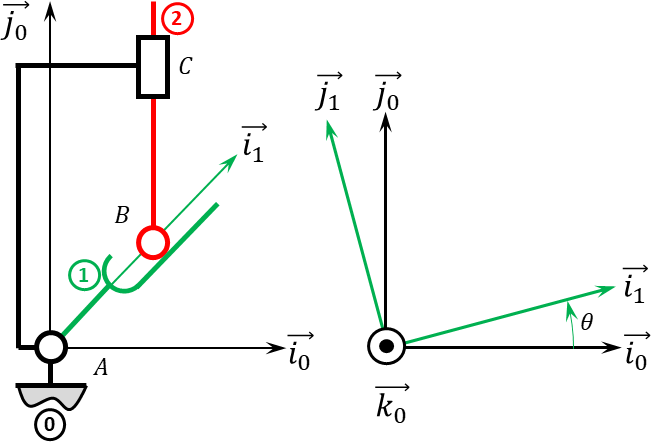
\includegraphics[width=\linewidth]{16_01}
\end{center}
\fi

\question{Tracer le graphe des liaisons.}
\ifprof
\else
\fi

\question{Exprimer $ \mu(t)$ en fonction de $\theta(t)$.}
\ifprof
\else
\fi

\question{Exprimer $\dot{\mu}(t)$ en fonction de $\dot{\theta}(t)$.}
\ifprof
\else
\fi

\question{En utilisant Python, tracer $\dot{\mu}(t)$ en fonction de $\dot{\theta}(t)$. On considérera que la fréquence de rotation de la pièce \textbf{1} est de 10 tours par minute.}
\ifprof
\else
\fi

\ifprof
\else
\begin{flushright}
\footnotesize{Corrigé  voir \ref{C2:06:16}.}
\end{flushright}%
\fi